%!TEX root = ../report.tex
\chapter{Methodology}
\label{chap:method}
\section{Data}
Just like any other machine learning project the data is the most important part of the evaluation. Hence for the proper qualitative evaluation a deeper look at the data and how it was generated is needed.
The data set for training and testing are both obtained from Valdenegro-Toro \cite{stateoftheart}. Following is a brief description of the overall pipeline to obtain the data for training.

\subsection{Sonar image capture procedure}
In Valdenegro-Toro \cite{stateoftheart} the authors have explained in details how the raw sonar images were captured. In a water tank in their facility, the images were taken using ARIS Explorer 3000 and
mounted Forward-Looking Sonar (FLS). The objects featured are household garbage items and common marine debris. There are total 9 different types, such as metal cans, bottles, drink carton, metal chain, propeller, tire, hook, valve. 
In \cite{stateoftheart}, in controlled underwater environment total of 2072 images; about 2500 instances of the aforementioned objects were captured and labeled with 9 classes accordingly.

\subsection{Data generation for deep learning}
\begin{figure}[ht]
\centering
\includegraphics[height= 8cm]{images/densenet/training_data_generation}
\caption{Algorithm for matching and non matching pair of patch generation from Valdenegro-Toro \cite{stateoftheart}}
\label{fig:training_data_generation}
\end{figure}

As part of the same work \cite{stateoftheart}, matching and non-matching pairs 
of sonar image patches were generated using a patch generation algorithm displayed in figure \ref{fig:training_data_generation} where each patch, an instance of one of the 9 classes, were obtained from meaningful crops of the original 
sonar images. Authors have figured that 96x96 pixels is the best size of the crops.

\begin{figure}[ht]
\centering
\includegraphics[width= 14cm]{images/densenet/data_pipeline2}
\caption{Data processing pipe line}
\label{fig:data_pipeline}
\end{figure}

To create matching pair, two patches that belong to the same object-type but different perspective and insonification level were used. For generating non-matching pair, two instances of different 
object-types were used. Also, one instance of an object and a background patch, which contains no object instance, were used to generate additional non-matching patches. According to the authors of \cite{stateoftheart}, 
for balanced and effective learning, the ratio of matching and non-matching pairs in both train and test data is maintained at 1:1. That is, for every ten matching pair five object-object non-matching 
and five object-background non-matching pairs were generated. In figure \ref{fig:data_pipeline} the overall pipeline for the data generation is displayed in simple block diagram.
In figure \ref{fig:generated_patches} some sample patches from all type of pairs are displayed. Using the patch generation algorithm total of 
39840 pairs were generated from the instances of 6 distinct object type, which were used as the train data.
While another 7440 pairs were generated from the instances of remaining object types, for testing purpose. This test dataset does not contain any common object with the training dataset,
it should be a good test for the generalization of the approaches. The labels for the data are 0 and 1 representing non-matching and matching pairs respectively. 
For this thesis work, this dataset is obtained in HDF5 files \cite{hdf5}. It contains patches in form of tensors \cite{tensors}, each of shape (2,96,96). Here the pair of patches (size 96x96) are placed in a way that each channel
contains one patch. %For final comparison of performance the same test data will be used.

\begin{figure}[ht]
\centering
\includegraphics[height= 13cm]{images/densenet/generated_patches}
\caption{Some sample of the matching and non-matching pairs from Valdenegro-Toro \cite{stateoftheart}}
\label{fig:generated_patches}
\end{figure}

\flushbottom
\newpage
\section{Architecture To Be Evaluated}
\label{architectures}

In this section the theoretical aspect of the different architectures that we are using are explained along with brief implementation details where applicable. %TODO mention the sources of the implementations
\subsection{DenseNet two channel network}
In DenseNet each layer connects to every layer in a feed-forward fashion. 
With the basic idea to enhance the feature propagation, each layer of DenseNet blocks takes the feature-maps of the previous stages as input.  

The DenseNet implementation used is from the keras community contributions (keras\_contrib)  \cite{kerasdensenet}. Another DenseNet implementation was initially evaluated from Thibault de Boissiere \cite{densenetold}, but it was older 
implementation and did not have bottleneck or compression implemented. 

\begin{figure}[ht]
\centering
\includegraphics[width=0.5\textwidth]{images/densenet/densenet.png}
\caption{Example DenseNet architecture from \cite{densenet}.}
\label{fig:densenet}
\end{figure}

In DenseNet two channel the the sonar patches are supplied as inputs in two channels format, the network by itself divides each channel into one patch and learn the features from the patches and then finally compare them using the Sigmoid 
activation function at the end with FC layer of single output. The original label in the data is 0 for non-matching pair of input patches. Label 1 means matching pair.

DenseNet architecture depends on the hyperparameter settings of the instantiation. The parameters and their brief definition is described in the following section. 
\begin{itemize}
  \item \textbf{Growth rate}: Number of filters to add per dense block. Growth rate regulates how much information is contributed by each layers to the global state. 
  Global state is the collective knowledge of the network, that is the state of the previous layers are flown into each layer in form of feature-maps, 
  which is considered as global state. Each layer adds k more feature-maps to the current state, when growth rate is k.

  \item \textbf{Nb\_filter}: initial number of filters. -1 indicates initial number of filters will default to 2 * growth\_rate.

  \item \textbf{Nb\_layers\_per\_block}: number of layers in each dense block. Can be a -1, positive integer or a list. If -1, calculates nb\_layer\_per\_block from the network depth. 
  If positive integer, a set number of layers per dense block. If list, nb\_layer is used as provided. Note that list size must be nb\_dense\_block.

  \item \textbf{Depth}: number or layers in the DenseNet.

  \item \textbf{Nb\_dense\_block}: number of dense blocks to add to end.

  \item \textbf{Bottleneck Layers}: To improve computation efficiency a bottleneck layer with 1x1 convolution is introduced before each 3x3 convolution layers. 
  \item \textbf{Compression}: Reduces the feature maps in transition layers and makes the model more compact and computationally efficient.
\end{itemize}

\newpage
\subsection{DenseNet-Siamese Network}

In this architecture the branches of the Siamese network are DenseNet. Following the classic Siamese model the branches shares weights between them and gets trained simultaneously on two input patches and then learns the features from the inputs.
Through the shared neurons it the Siamese network is able to learn the similarity function and be able to discriminate between the two input patches. The role of the DenseNet branches are feature extraction, the decision making or prediction 
part is taken care of by the Siamese network.

\begin{figure}[ht]
\centering
\includegraphics[width=0.5\textwidth]{images/densenet/siamese_densenet_structure.png}
\caption{DenseNet-Siamese architecture.}
\label{fig:dn_siamese}
\end{figure}

In figure \ref{fig:dn_siamese} the basic architecture is displayed for the DenseNet-Siamese network. The two DenseNet branches are designed to share weights between them. The extracted features are concatenated and connected through a
FC layer, followed by activation Relu and where applicable Batch normalization and dropout layers. The output is then connected to another FC layer with single output, for binary prediction score of matching (1) or non-matching (0). 
Sigmoid activation function and binary cross entropy loss function is used for this final FC layer. As mentioned in the figure \ref{fig:dn_siamese} the size of the output of the FC layer (f) and value of dropout probability etc. hyperparameters
are to be decided after thorough hyperparameter search.

\newpage
\subsection{Contrastive Loss}
Using Contrastive loss higher dimensional input data (e.g. pair of images) can be mapped in the much lower dimensional output manifold, where similar pairs are placed closer to each other and 
the dissimilar pairs have bigger distances between them depending on their dissimilarity.  So using this loss function the “distance” between two input patches projected in the output manifold can be 
predicted and if the distance is closer to 0 then the input pairs are matching, otherwise its dissimilar (above threshold). The formula for the loss is shown below. 
\begin{figure}[ht]
\centering
\includegraphics[height= 0.45cm]{images/contrastive/contrastive_loss_formula1.jpg}%TODO exchange this with the actual latex code
\label{fig:contrastive_loss_formula1}
\end{figure}

\begin{figure}[ht]
\centering
\includegraphics[height= 0.7cm]{images/contrastive/contrastive_loss_formula2.jpg}
\label{fig:contrastive_loss_formula2}
\end{figure}

Here L is the loss term, the formula presented here is the most generalized form of the loss function, suitable for batch training. 
$ \vec{X_1}$, $ \vec{X_2}$ represents a pair of input image vectors. Y are the labels, 0 for similar pair and 1 for dissimilar pair. $D_w$ is the parameterized distance function to be learned by the algorithm. 
m is the margin and m is always greater than zero and it defines a radius around $G_w$. The dissimilar pairs only contribute to the loss function if their distance is within the radius.
One of the idea for evaluating this loss function is to use it with a Siamese network, as the loss function takes a pair of images as input. So its very relevant to the problem statement of this thesis. 

%\newpage

\subsection{VGG-Siamese Network}

The VGG network \cite{VGG} is a CNN which was conceptualized by K. Simonyan and A. Zisserman from the University of Oxford (Visual Geometry Group). This network performed very well in ImageNet challenge 2014. The architecture/s has 
very small 3x3 Conv filters and depth varying from 16 to 19 weight layers. This network became very popular because it generalize very well for different kinds of data, which is very reason this is network is chosen for evaluation.

\begin{figure}[ht]
\centering
\includegraphics[width=14cm]{images/contrastive/VGG_network_structure}
\label{fig:VGG_network_structure}
\caption{VGG network structure. At the end of the network structure there are two fully-connected or dense layers, will also evaluate if more or less number of dense layers are required
The number of dense layers at the end is also a hyperparameter denoted by l.}
\end{figure} 

The basic VGG network structure, i.e each branch of Siamese is as follows, \code{Conv(n, a x a)-Conv(n, a x a)-MP(2, 2)-Conv(2n, a x a)-Conv(2n, \\a x a)-MP(2, 2)-Conv(4n, a x a)-Conv(4n, a x a)-Conv(4n, a x a)-\\MP(2, 2)-Conv(8n, a x a)-Conv(8n, a x a)-
Conv(8n, a x a)-MP(2, 2)-\\Conv(8n, a x a)-Conv(8n, a x a)-Conv(8n, a x a)-MP(2, 2)-FC(d)-FC(d)}. The a, n and d are hyperparameters which needs to be optimized. The details of the evaluation is presented in the \autoref{sec:contrastive_loss_results}.
The implementation is acquired from Fabio Perez \cite{vggimpl}.

\begin{wrapfigure}[13]{l}{6cm}
\hspace{1cm}
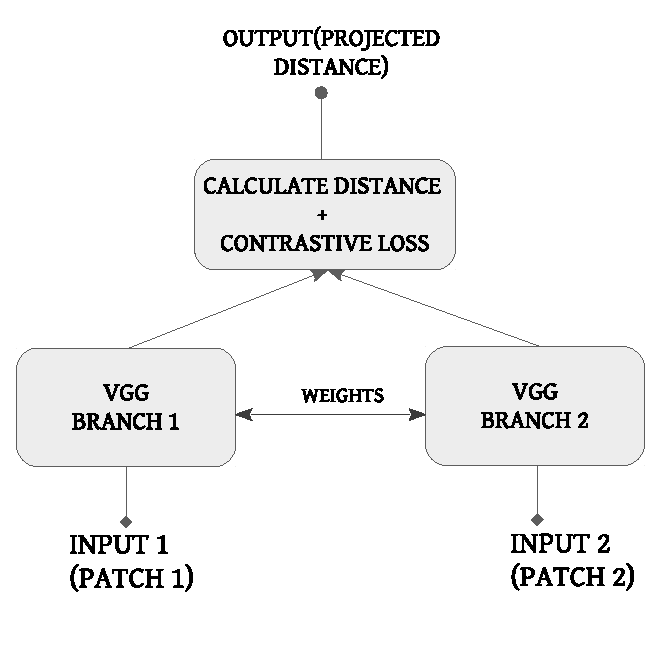
\includegraphics[height=6cm,width=5cm]{images/contrastive/siamese_contrastive_loss}
\caption{VGG Siamese network with contrastive loss}
\label{fig:network_structure_vgg_siamese}
\end{wrapfigure} 

To evaluate the Contrastive loss a Siamese network has been selected since it also takes two input images and compare them. For the branch structure of the Siamese (figure \ref{fig:network_structure_vgg_siamese}) VGG network 
has been chosen. The role of the VGG network \cite{VGG} is to extract features, similar to the DenseNet-Siamese, the final decision making and prediction is taken care of by the Siamese network. In this case the output is
actually euclidean distance between the two input sonar patches, projected into lower dimension using Contrastive loss.




